\section{Inside the SST Tool: Registration, Data Integration, and Storage}\label{sec:sst_tool}

We have already discussed at length that data extracted from the probes can be plugged into the SST tool, which works as a unified data source. We will explore the SST tool in this section, its purpose, and how it operates. We will begin by discussing how to run this tool. After that, we will examine the types of data that its endpoints accept, ensuring that we implement our probes correctly according to the REST API structure.

In later subsections, we will focus on how data is collected from probes, how it is sent to the SST tool, and finally, how it is stored. This step-by-step breakdown will help us understand the complete workflow, from data input to storage.

\subsection{Running the SST Tool}

The SST tool depends on two main services:  
\begin{itemize}
    \item \textbf{SST Backend Service} – This service is responsible for sending and receiving probe data.
    \item \textbf{Neo4j Database} - This database stores the collected data in a graph-based format, making it easier to visualize and analyze relationships between data points.
\end{itemize}

To set up SST, we first need to clone the source code from the GitHub repository~\citep{uds_github}. After cloning, we require a docker compose file to initialize and run these services. The necessary and up-to-date docker-compose file is available on Docker Hub~\citep{sst_dockerhub}. By using this setup, we ensure that all components of the SST tool are properly configured and ready for use.

Once both of the above steps are completed, run the services using ``docker-compose up''. We can check the backend services running by sending a get request to this URL: \texttt{localhost:8000/api/health-check}.

\subsection{Probe Registration}

All probes must be registered first to ensure that the data remains consistent. The registration process ensures that the SST system can correctly store, process, and relate the incoming data. To register a probe, the following three elements are required:

\begin{itemize}
    \item \textbf{Probe Name} – The name of the probe that is being registered.
    \item \textbf{Nodes} – The data elements that will be provided to the SST system.
    \item \textbf{Edges} – The relationships between the nodes.
\end{itemize}

Each node represents an object that holds specific data. It is important that each node is unique and contains a value that serves as its unique identifier. This identifier is crucial because SST merges nodes based on this value. If a node with the same identifier already exists in the system, the original one will be retained, preventing duplication.

Edges define how nodes are connected to each other, establishing relationships between them. These relationships help structure the data in a meaningful way, allowing for efficient querying and retrieval within the system.

\begin{figure}[H]
    \centering
    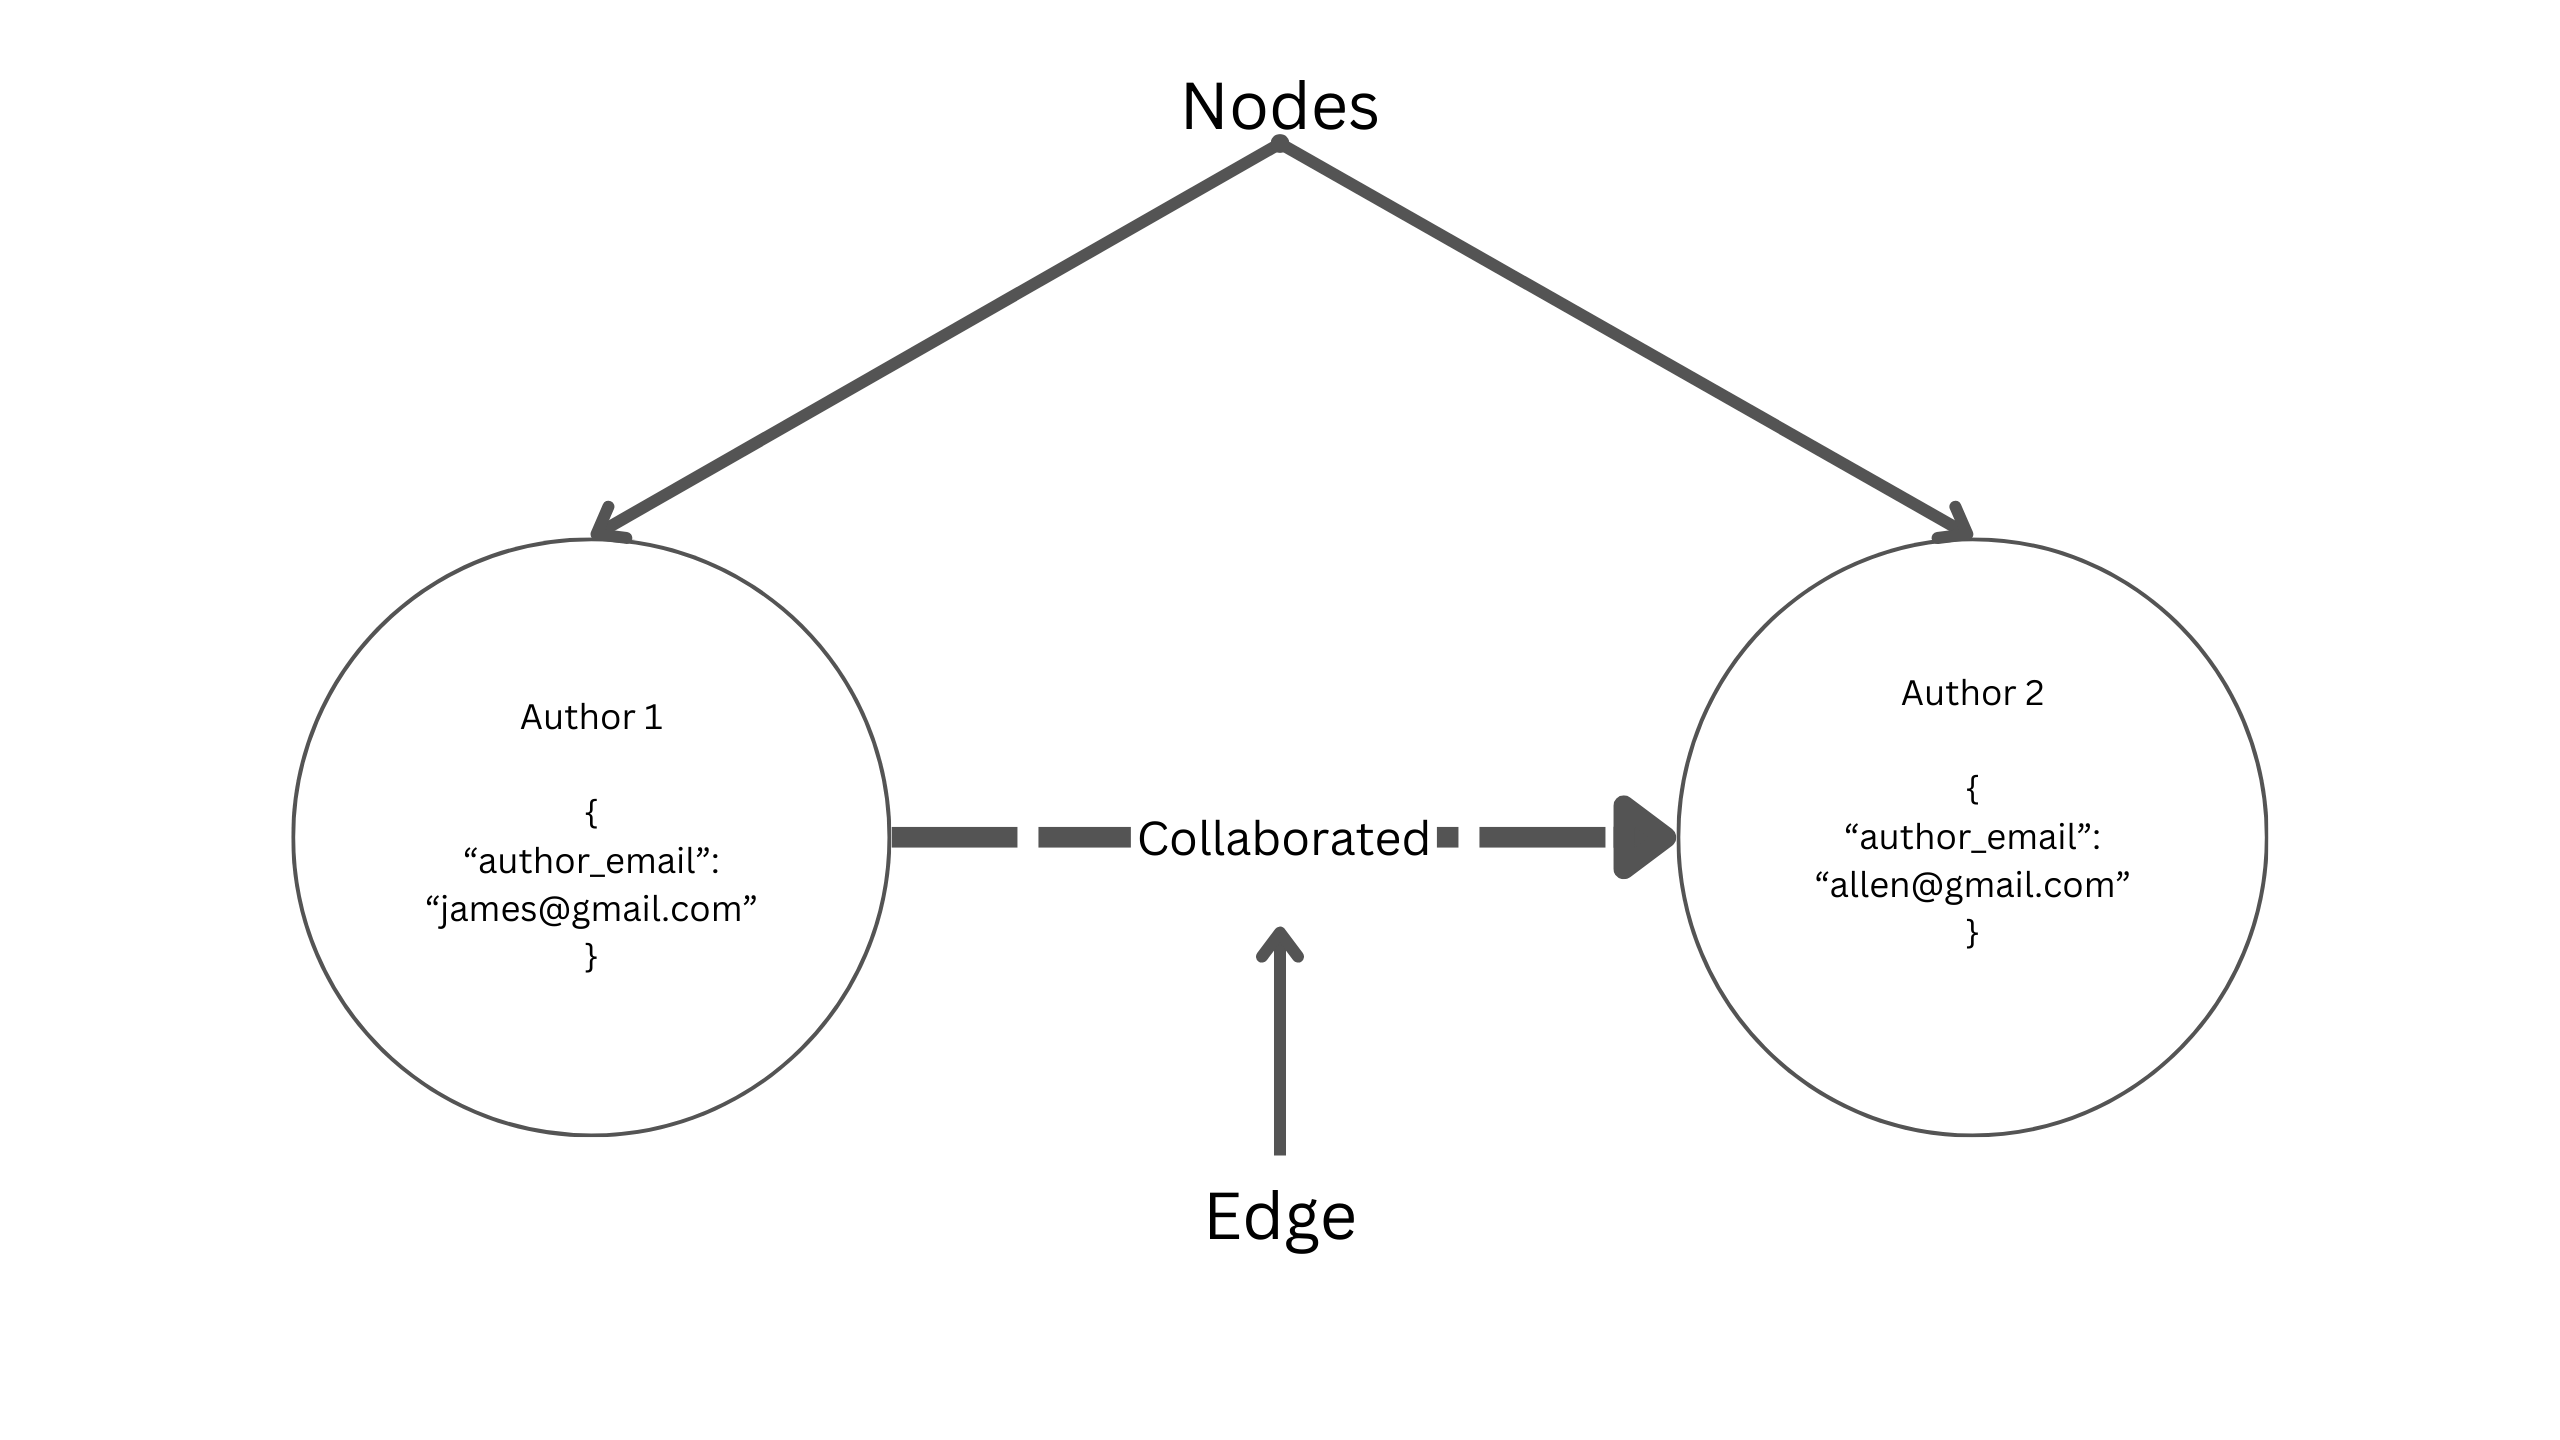
\includegraphics[width=1\textwidth]{figures/nodes_and_edges.png}
    \caption{Nodes and Edges}
    \label{fig:nodes_and_edges}
\end{figure}

\begin{figure}[H]
    \centering
    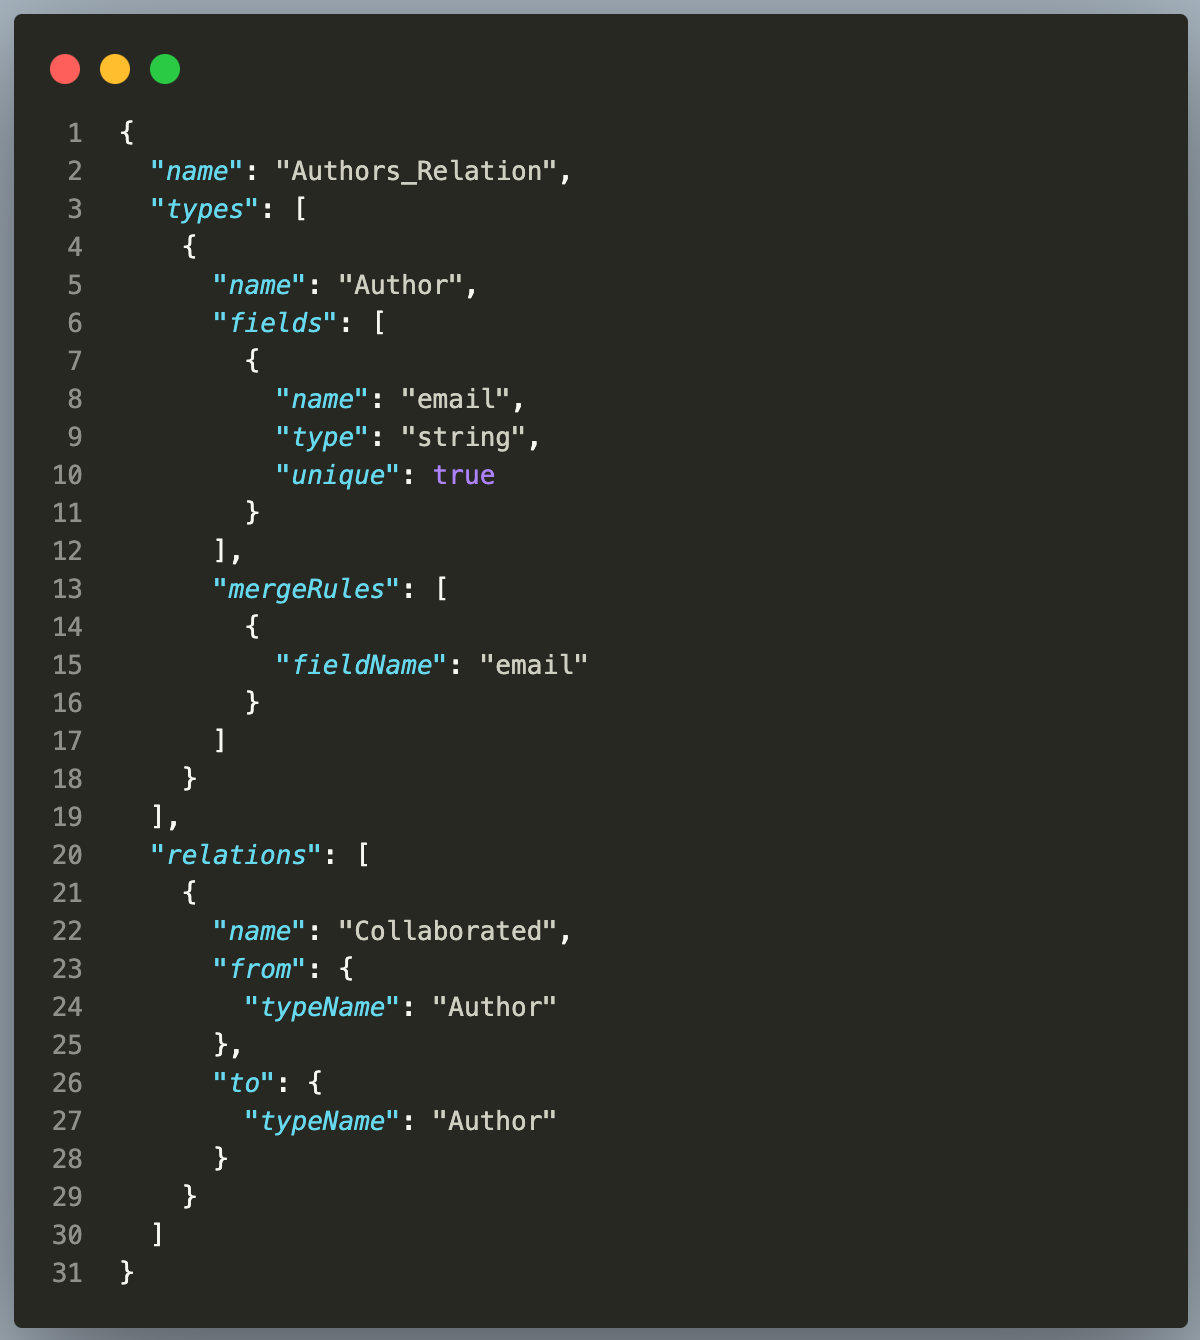
\includegraphics[width=0.50\textwidth]{figures/author_relation.png}
    \caption{JSON for Author Relation Probe Registration}
    \label{fig:json_author_relation}
\end{figure}

Figure~\ref{fig:json_author_relation} shows the JSON required to register a probe. ``types'' is an array of JSON objects, where each object in this array represents a node type. Each node has a ``name'', an array of ``fields'', and ``mergeRules''. The ``fields'' represent the object attributes for the node, while ``mergeRules'' define the value on the basis of which two nodes will be merged.  

``relations'' is another array of JSON objects, where each object represents a relationship between two nodes. Each relation has a ``name'', a ``from'' field, and a ``to'' field. The ``from'' and ``to'' fields define the node types between which the relationship should be established. This structure ensures that data is correctly linked within the SST system, allowing for efficient merging and retrieval of information.

Once the structure of the probe is defined, it must be registered using the following REST API provided by the SST tool. Use post request and send the JSON data to the SST. If the probe is registered, it will return a response status code of 201 and a status of ``success'' will be shown in the response object.
\begin{lstlisting}[language=bash]
localhost:8000/api/probes
\end{lstlisting}

\subsection{Probe Integration}

Once the probe has been registered, the next process is to extract the data from the source code for integration with SST. Make sure the data should be in the same structure as the structure that is used to register the probe. 

\begin{figure}[H]
    \centering
    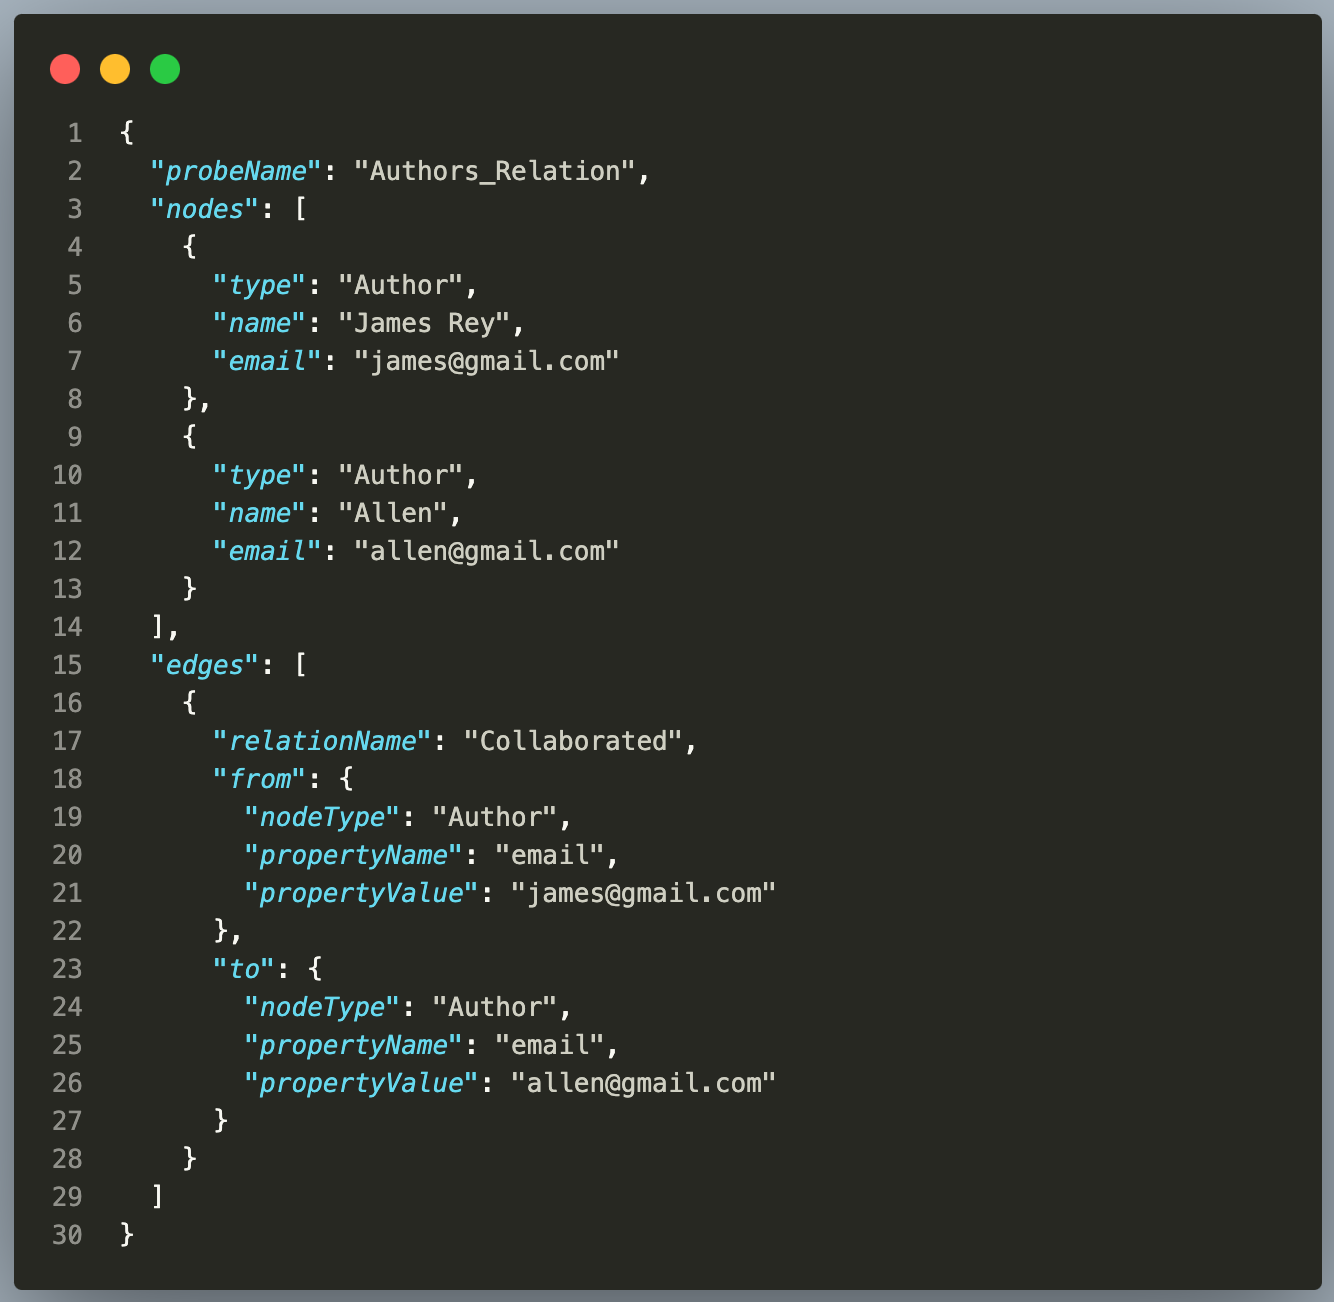
\includegraphics[width=0.60\textwidth]{figures/author_relation_int.png}
    \caption{JSON for Author Relation Probe. It represents the same scenario as shown in~\ref{fig:nodes_and_edges}}
    \label{fig:json_author_relation_int}
\end{figure}